\documentclass[]{article}
\usepackage[backend=biber, style=apa]{biblatex}
\usepackage{paralist}
\usepackage{hyperref}
\usepackage{float}
\usepackage{graphicx}
\usepackage{booktabs}
\usepackage[toc,page]{appendix}
\usepackage[margin=2.5cm]{geometry}
\graphicspath{ {./images/} }

\addbibresource{report.bib}
\newtheorem{researchquestion}{RQ}

%opening
\title{A YOLOv8-based Analysis of Image Augmentation Techniques for Vehicle Detection in Adverse Weather Conditions}
	\author{
		Alexander Van Hecke \small(852631385) \and 
		Frederik Lefever    \small(838836963)}

\begin{document}

\maketitle

\begin{abstract}
	Vehicle detection in images is a necessary condition for semi-automated traffic monitoring.  We investigated whether image augmentation can be used to increase the accuracy of vehicle detection in images of adverse weather conditions. We created two vehicle detection models, both derived from a standard YOLO\small{v8} model. One model was produced from actual adverse weather traffic images, the other model from augmented traffic images. We compared the accuracy of our models with that of the untrained  YOLO\small{v8} model and one against the other. Our initial expectation was that the trained models would both outperform the untrained model and were interchangeably accurate. We found that a significantly higher accuracy could be obtained from training with actual adverse weather images, but observed no such improvement from applying image augmentation. The artefacts of this study are made available at \cite{Van_Hecke_YOLOv8-based_Analysis_of_2024}.
\end{abstract}

\section{Introduction}

	Adverse weather conditions such as rainfall, snow and fog are known to have an effect on traffic flow. Traffic breakdown occurs when demand exceeds capacity in some part of a transportation network and in \cite{stralenInfluenceAdverseWeather2015} it is shown that the odds of traffic breakdown at bottleneck locations are significantly increased by rainfall.  This can lead to considerable economic damage and provides a strong incentive to mitigate this problem as much as possible.
	
	Traffic monitoring and dynamic flow control can be part of a mitigation strategy. The current technology behind traffic monitoring largely uses vehicle detection in images captured from CCTV cameras positioned next to highways. However, vehicle detection in images deteriorates in the presence of noise from adverse weather conditions.
	
	We investigated the effect of image augmentation on the robustness of YOLO{\small v8}-based vehicle detection models. In particular, we investigated the effect of artificially adding rain, fog and snow to clear weather images of traffic situations. Compared to the standard YOLO{\small v8} model, we expected to see an improvement in the accuracy of the number of cars and buses detected. To estimate how well training with image augmentation can approximate training with actual adverse weather images, we produced a second model from actual images. The accuracy of this model was then compared with both the standard YOLO{\small v8} model and the model obtained from augmented images.
	
	We chose YOLO{\small v8} because of its popularity in both academia and industry. YOLO{\small v8} is well-documented, both as a ready-to-use product and in scientific literature. It is an open-source software, licensed under AGPL-3.0. For the augmentation of images, we chose Imgaug by \cite{imgaug} and to train the standard YOLO{\small v8} we chose Google Collab (\url{https://colab.research.google.com/}).

\section{Literature review}

	In the context of machine learning, image augmentation can broadly be defined as the automated creation of variation in actual image datasets. Large volumes of data with sufficient variation can alleviate the problem of overfitting. Yet sometimes sampling data from an application domain is nontrivial, eg. when learning from medical images.  Image augmentation can be used to artificially create additional images, or to add some sort of noise to images in order to make the resulting model more robust.
	
	A comprehensive survey of modern image augmentation techniques is presented in \cite{shortenSurveyImageData2019}. Several approaches such as geometric transformations, color space augmentations, kernel filters, mixing images, random erasing, feature space augmentation, adversarial training, generative adversarial networks, neural style transfer, and meta-learning, are explained.  A more recent survey of image augmentation techniques as used in deep learning is presented in \cite{xuComprehensiveSurveyImage2023} . This survey introduces a novel taxonomy, where image augmentation algorithms are classified as either model-free, model-based, or optimizing policy-based. The objectives of image augmentation are explained by analysing the challenges encountered when deploying deep learning models for computer vision. A theoretical framework for understanding data augmentation is described in \cite{daoKernelTheoryModern2019}. First a general model of augmentation as a Markov process is given, and it is shown that kernels appear naturally with respect to this model. Next, a more direct analysis of the effect of augmentation on kernel classifiers is offered.
	
	The effectiveness of image augmentation on the classification of images with deep learning is discussed in \cite{perezEffectivenessDataAugmentation2017}. Simple techniques, such as cropping, rotating, and flipping images are compared. Additionally this paper reports on experiments with generative adversarial neural networks to learn augmentation strategies.
	
	Research similar to our research can be found in \cite{kumarObjectDetectionAdverse2023}. The central question in \cite{kumarObjectDetectionAdverse2023} is whether YOLO{\small v8} can be improved through transfer learning to detect objects in adverse weather. This paper supports the hypothesis that training with actual images of adverse weather conditions significantly improves the detection performance compared to the standard YOLO{\small v8} model. An enhanced YOLO\small{v8}-based model for vehicle detection in foggy weather conditions is the focus of \cite{liVehicleDetectionFoggy2022}. The approach used to create the enhanced model is interesting in that the training set is obtained from 350 traffic images that are augmented with a fog-effect and subsequently dehazed with the multi-scale retinex with color restoration (MSRCR) algorithm. The final training set is then composed of the original images, fogged images and dehazed images. Whereas results in \cite{liVehicleDetectionFoggy2022} are reported with autonomous vehicles in mind, \cite{songVisionbasedVehicleDetection2019} specifically targets vehicle detection and counting in highway management.  A new segmentation method is proposed to divide a depicted highway road surface into a distal and a proximal area. Using this separation a YOLO{\small v3} model is trained to detect the type and location of vehicles. To estimate vehicle count and trajectories the Oriented FAST and Rotated BRIEF (ORB) algorithm is added to the image processing pipeline.
	

\section{Research questions}

	Many image augmentation techniques are described in the literature, ranging from simple geometric transformations to the addition of noise and changing colour, saturation and hue parameters. We investigated the effect of \textit{thematic} image augmentation, meaning that we added artificial rain, fog and snow to clear weather images. At the more general level, we aimed to answer following questions:

	\begin{researchquestion}
	\label{rq1}
	Given that the standard YOLOv8 model is used as a reference model and a new	model is derived from it by transfer learning with thematically augmented images,	will the new model then more accurately predict the number of vehicles in actual images	of traffic in adverse weather conditions?
	\end{researchquestion}

	Furthermore, to appreciate the value of image augmentation in contexts where data is not necessarily scarce, we pose two additional questions:
	\begin{researchquestion}
	\label{rq2}
	Given that the standard YOLOv8 model is used as a reference model and a new model is derived from it by transfer learning with actual images of traffic in adverse weather conditions, will the resulting model then more accurately predict the number of vehicles in actual images of traffic in adverse weather conditions?
	\end{researchquestion}

	\begin{researchquestion}
	\label{rq3}
	Given two models, each obtained by transfer learning the standard YOLOv8 model on an identical number of images. One model is learned from thematically
	augmented images, the other model from actual images of traffic in adverse weather conditions. Will both models then make predictions with comparable accuracy about the number of vehicles in actual images of traffic in adverse weather conditions?
	\end{researchquestion}

	Informally, the third research question asks whether learning from actual images can be replaced with learning from thematically augmented images without significantly changing the expected accuracy of the obtained model. Central to the concept of accuracy used in each of the above three research questions is the intersection over union (IoU) metric. This metric compares predicted bounding boxes with verified bounding boxes (the latter being referred to as “ground truth”). We use the IoU as a numeric representation of the presence or absence of vehicles in images and to calculate
	statistical significance of the learning effects.	

\section{Research method}

\subsection{Datasets}

	Two open-source datasets are used for this research. The DAWN dataset \cite{bw1x-yh39-20} is a collection of 1000 images from real-traffic environments in adverse weather conditions. The images are divided into four sets of weather conditions: fog, snow, rain and sandstorms. They are annotated with object bounding boxes and are labelled.  The second dataset is the UA-DETRAC \cite{CVIU_UA-DETRAC} dataset. This dataset provides 140K traffic images taken at Beijing and Tianjin (China). Images of the UA-DETRAC dataset are divided into four weather categories: ``cloudy'', ``night'', ``sunny'' and ``rainy''. They are annotated with object bounding boxes and are labelled.  We focused on the common labels between these two datasets, ``car'' and ``bus''.

\subsection{Model selection}
 
	For vehicle detection we chose an open source convolutional neural network called YOLO{\small v8} \cite{yolov8_ultralytics}. We use this model in transfer learning and as a reference for derived models. YOLO{\small v8} is trained on the Microsoft COCO dataset \cite{linMicrosoftCOCOCommon2015a} and capable of detecting object categories ``car'' and ``bus''.  Several sizes of the YOLO{\small v8} model are available, ranging from a ``nano'' model to a ``large'' model.  We started from the ``large'' model in all experiments, and trained it for 300 epochs.  This is the minimum number of epochs suggested by the authors of the YOLO{\small v8} model.

\subsection{Experiments}

	From the DAWN dataset, only images containing at least one of the common labels (``car'', ``bus'') were kept.  Sandstorm images were not kept, as this was not something we could artificially generate using the chosen augmentation software imgaug \cite{imgaug} (version 0.4.0).  This resulted in 698 images, which were first shuffled randomly and then split in a training set of 501 images (about 70\%), a validation set of 99 images (about 15\%), and a test set of 98 images (about 15\%).

	From the UA-DETRAC dataset, only images taken in sunny conditions were kept.  As the goal was to artificially augment these images, we wanted to start from the best weather condition possible.  These images were shuffled randomly and a selection of 167 training images and 33 validation was made.  Each of those images was then artificially augmented with a fog effect, a snow effect (flake size $[0.8 - 1.0]$, speed $[0.01 - 0.05]$), and a rain effect (drop size $[0.4 - 0.8]$, speed $[0.3 - 0.8]$).  This resulted in a training set of $3 \times 167=501$ images, and a test set of $3 \times 33=99$ validation images, the same number of images as in the training and validation sets of the DAWN dataset.  See Table \ref{table:datasets} for an overview, and Figure \ref{fig:example-images} for examples of images from the DAWN and UA-DETRAC datasets (both with and without augmentation).

\begin{table}[H]
	\centering
	\begin{tabular}{cccrrrp{1.5in}}
		\toprule
		\textbf{dataset} & \textbf{relevant labels} & \textbf{filter} & \textbf{training} & \textbf{validation} & \textbf{test} \\
		\midrule
		\textbf{DAWN} & car, bus & fog, snow, rain & 501 & 99 & 98  \\
		\textbf{UA-DETRAC} & car, bus & sunny &  501 & 99 &  \\
		\bottomrule
	\end{tabular}
	\caption{Datasets used}
	\label{table:datasets}
\end{table}

\begin{figure}
	\begin{tabular}{cc}
		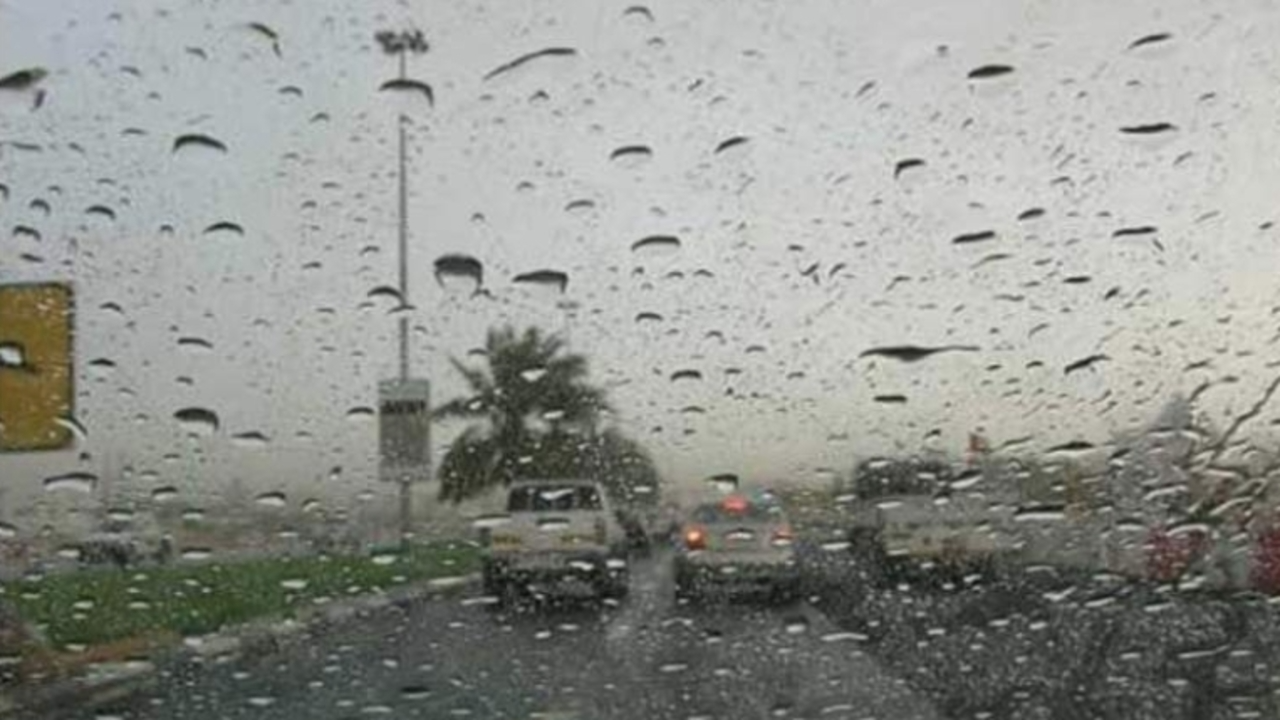
\includegraphics[width=65mm, height=40mm]{dawn-train-fullres.png} &   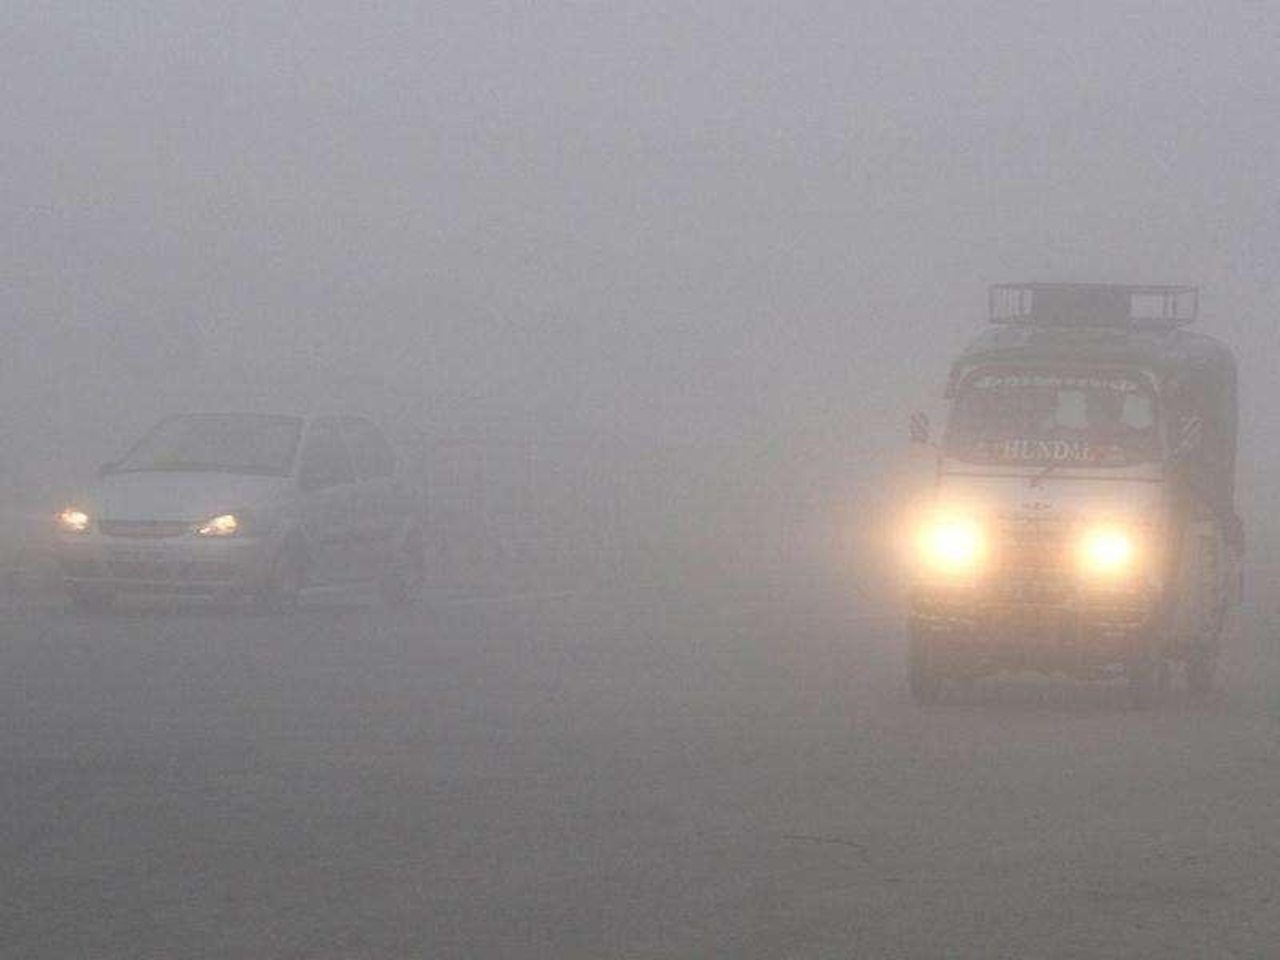
\includegraphics[width=65mm, height=40mm]{dawn-fog.jpg} \\
		(a) DAWN rain & (b) DAWN fog  \\[6pt]
		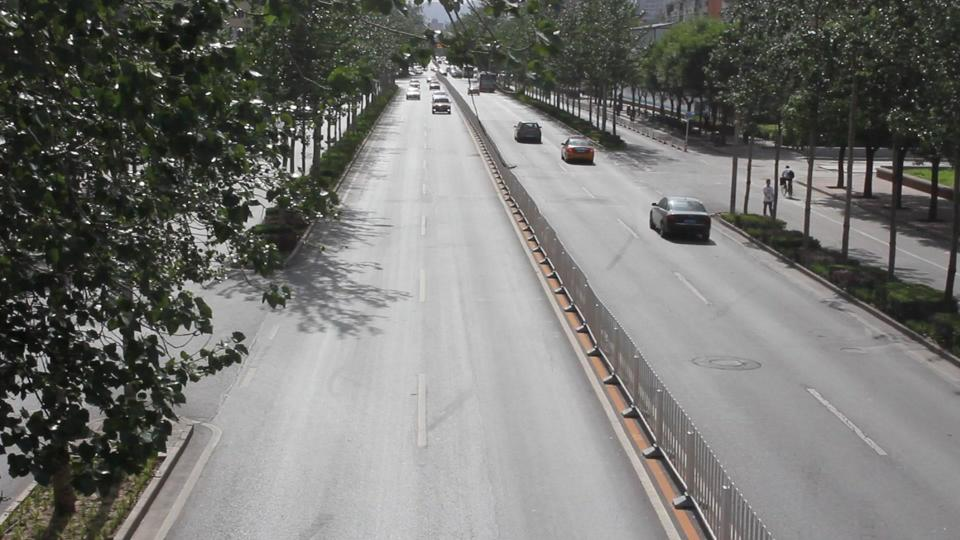
\includegraphics[width=65mm, height=40mm]{detrac-orig.jpg} &   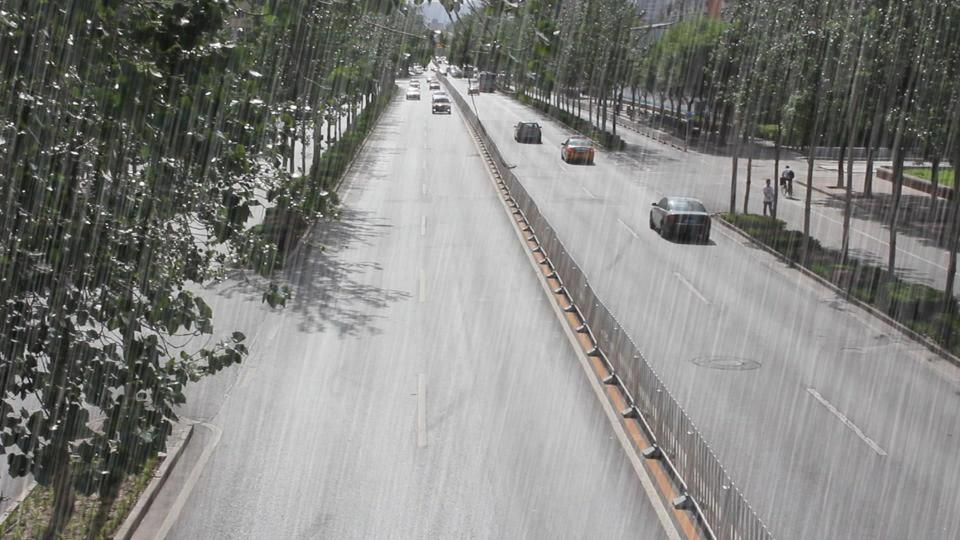
\includegraphics[width=65mm, height=40mm]{detrac-rain-fullres.png} \\
		(c) UA-DETRAC original  & (d) UA-DETRAC augmented rain \\[6pt]
		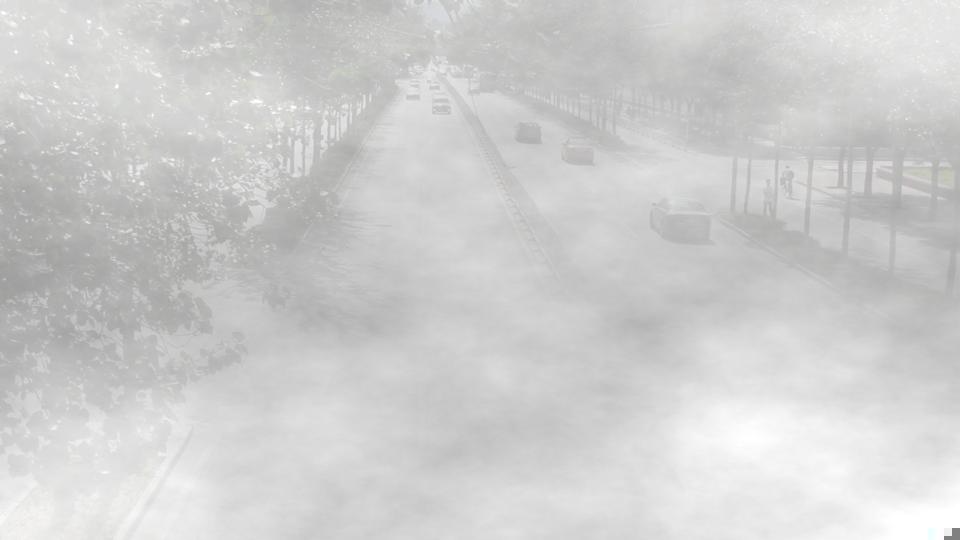
\includegraphics[width=65mm, height=40mm]{detrac-fog-fullres.png} &   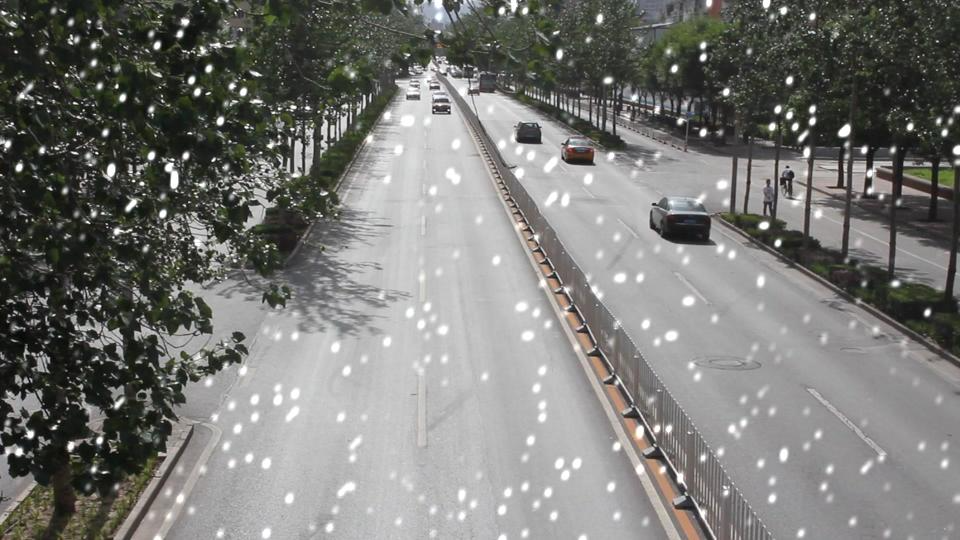
\includegraphics[width=65mm, height=40mm]{detrac-snow-fullres.png} \\
		(c) UA-DETRAC augmented fog & (d) UA-DETRAC augmented snow \\[6pt]
	\end{tabular}
	\caption{Example images of the DAWN and UA-DETRAC datasets.  (a) contains a rainy image in the DAWN dataset, (b) a foggy image in the DAWN dataset.  (c) contains an original image in the UA-DETRAC dataset (sunny conditions).  This UA-DETRAC image is artificially augmented with rain (d), fog (e) and snow (f)  }
	\label{fig:example-images}
\end{figure}

	To establish a baseline measurement, we took the out-of-the-box large YOLO{\small v8} model and used it to do predictions against the test dataset taken from DAWN (adverse weather images).  To answer the first research question \ref{rq1}, we trained a large YOLO{\small v8} model using the training and validation dataset taken from UA-DETRAC (augmented images) for 300 epochs.  This model was used to do predictions against the test dataset taken from DAWN (adverse weather images).  To answer the second research question \ref{rq2}, we trained a large YOLO{\small v8} model using the training and validation dataset taken from DAWN (adverse weather images) for 300 epochs.  This model was used to do predictions against the test dataset taken from DAWN (adverse weather images).  This is summarized in Table \ref{table:setuprq}.

\begin{table}[H]
	\centering
	\begin{tabular}{lll}
		\toprule
		\textbf{research question} & \textbf{training and validation} & \textbf{test} \\
		\midrule
		RQ1 & UA-DETRAC (thematically augmented images) & DAWN (adverse weather images) \\
		RQ2 & DAWN (adverse weather images) & DAWN (adverse weather images) \\
		\bottomrule
	\end{tabular}
	\caption{setup RQ \ref{rq1}}
	\label{table:setuprq}
\end{table}
\section{Data analysis}

	We believe our study can be classified as a single case mechanism experiment. In particular, we investigate the effect of differences in an independent variable $X$ taken from the set of object detection models, on a dependent variable $Y$ being the number of correctly detected cars and buses. Since we only consider three models (standard YOLO{\small v8}, a model derived from augmented images and a model derived from actual images), the study does not produce a volume of data large enough to use statistical inference. Results from presenting the DAWN test set to each of the three models are analysed by error rates and intersection over union (IoU).
	
\subsection{Error rates}
	
	The number of cars and buses predicted by each model are shown in Figure \ref{fig:counts}. The bars labelled ``Ground truth'' represent the actual number of cars and buses in the DAWN test set. With only 17 buses at ground truth, it seems unlikely that they will provide sufficient support for any of the observed effects. The analysis will hence focus more on the ``car'' category than the ``bus'' category.  
	
	\begin{figure}[h]
		\centering
		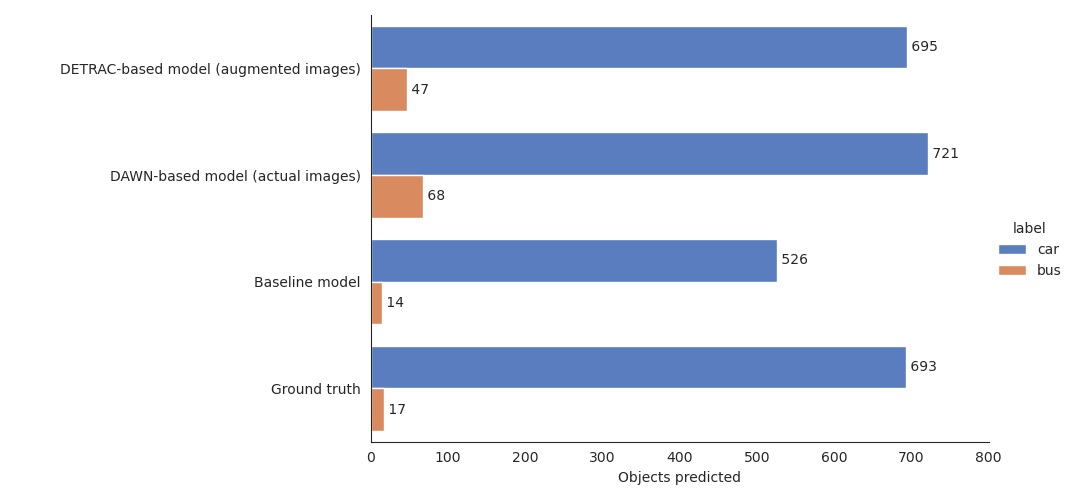
\includegraphics[width=120mm]{objectPredictionCounts.png}
		\caption{Number of cars and buses predicted by the object detection models versus ground truth.}
		\label{fig:counts}
	\end{figure}

	Error rates are calculated similarly to the bit error rate, with the ground truth number of each image as the centre value. For example, if ground truth specifies 8 cars for an image and the model only predicts 3, then the associated error rate is $\frac{8-3}{8}$ and if the model predicts 13 cars the error rate is $\frac{13-8}{13}$. The distribution of error rates is assumed to be normal. For the baseline, DAWN-based and DETRAC-based models, the distribution of error rates is given in Figure \ref{fig:error-rate-distributions}.
	
	\begin{figure}[H]
		\centering
		\begin{tabular}{lll}
			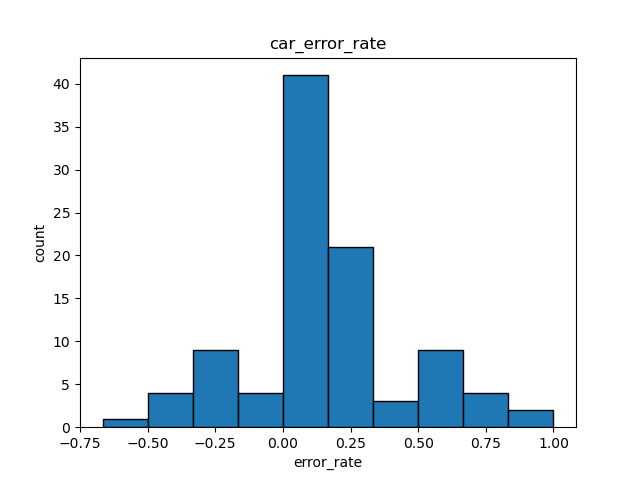
\includegraphics[width=60mm]{base_scenario_norm_car.png} & 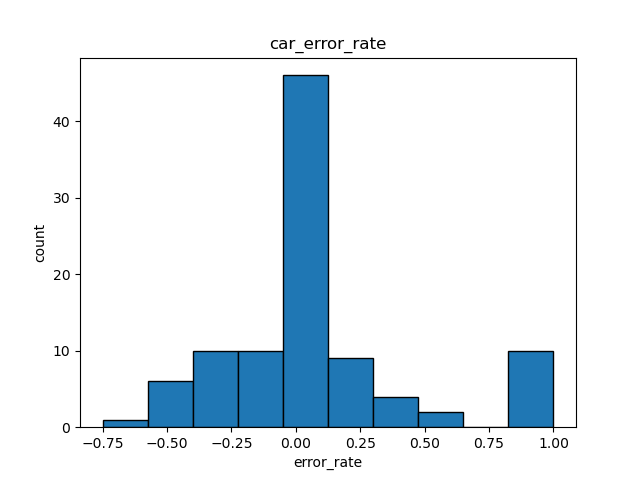
\includegraphics[width=60mm]{DAWN_scenario_norm_car.png} & 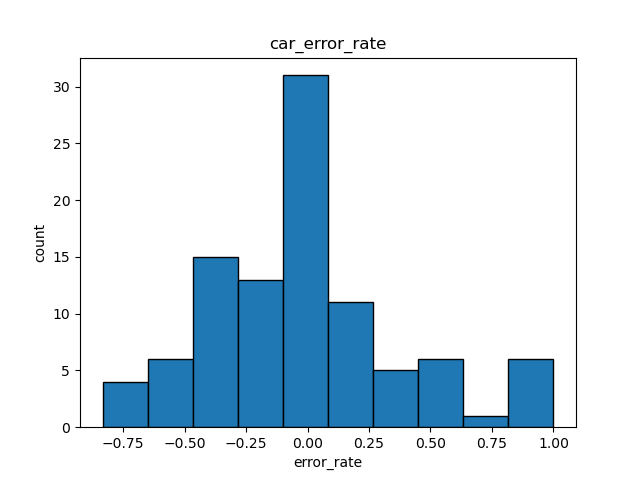
\includegraphics[width=60mm]{DETRAC_scenario_norm_car.png} \\
			(a) Baseline error rates & (b) DAWN error rates  &  (c) DETRAC error rates
		\end{tabular}
		\caption{Distribution of error rates obtained from the object detection models.}
		\label{fig:error-rate-distributions}
	\end{figure}
	
	
	To compare the mean error rates $\mu$, we performed a one-tailed paired t-test. Results are summarized in Table \ref{table:t-test}.	At the $\alpha=0.05$ significance level only the first null hypothesis can be rejected. Despite being below the $\alpha=0.05$ threshold, the p-values for the category ``bus'' provide little evidence in favour of either hypothesis.
	
	
	\begin{table}[H]
		\centering
		\begin{tabular}{ccrrp{1.5in}}
			\toprule
			\textbf{$H_0$} & \textbf{$H_a$} & Car p-value & Bus p-value \\
			\midrule
			$\mu\,\textsubscript{DAWN} = \mu\,\textsubscript{Baseline}$   & $\mu\,\textsubscript{DAWN} < \mu\,\textsubscript{Baseline}$   & 0.011 & 0.0   \\
			$\mu\,\textsubscript{DETRAC} = \mu\,\textsubscript{Baseline}$ & $\mu\,\textsubscript{DETRAC} < \mu\,\textsubscript{Baseline}$ &  0.109 & 0.0 \\
			$\mu\,\textsubscript{DAWN} = \mu\,\textsubscript{DETRAC}$ & $\mu\,\textsubscript{DAWN} < \mu\,\textsubscript{DETRAC}$ &  0.14  & 0.018 \\
			\bottomrule
		\end{tabular}
		\caption{One-tailed paired t-tests for mean error rates.}
		\label{table:t-test}
	\end{table}
	 
\subsection{Intersection over Union}  
	
	The analysis based on error rates is only indicative of accuracy \emph{at the image level}. With this measure of accuracy, it is possible to obtain maximum accuracy from completely erroneous predictions. For example, if the ground truth of an image specifies 8 cars and the model mistakenly classifies 8 trees as cars, then the error rate will be zero and the accuracy maximal. To make a more precise analysis, we used the intersection over union (IoU) as a measure of the accuracy of object detection. The IoU metric is used to evaluate the performance of object detection by quantifying the fit between the ground truth bounding box and the predicted bounding box. This idea is illustrated in Figure \ref{fig:iou}.
	
	\begin{figure}[h]
		\centering
		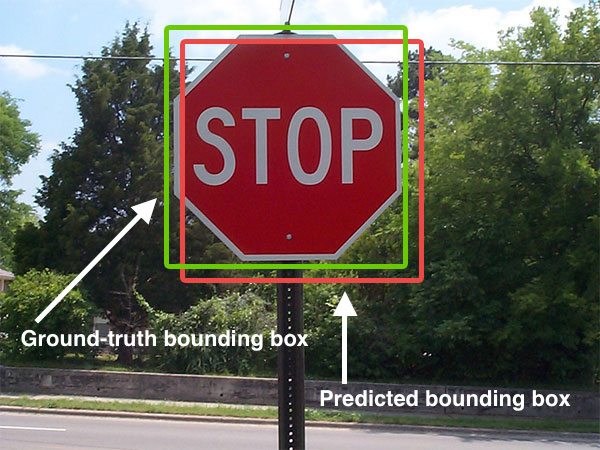
\includegraphics[width=5cm]{Intersection_over_Union_-_object_detection_bounding_boxes.jpg}
		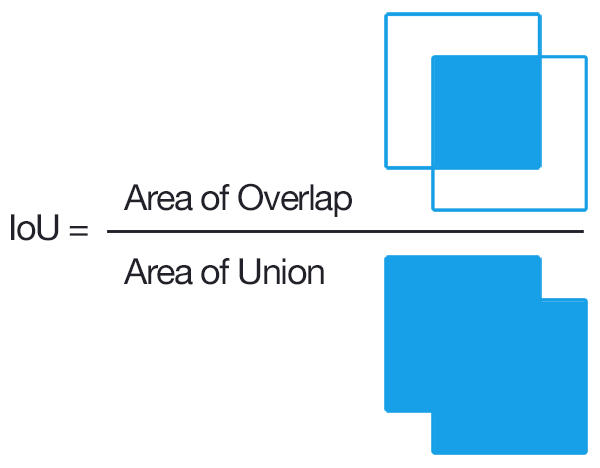
\includegraphics[width=5cm]{Intersection_over_Union_-_visual_equation.png}
		\caption{Images from Wikipedia \footnotesize{(\url{https://en.wikipedia.org/wiki/Jaccard_index})}}
		\label{fig:iou}
	\end{figure}
	
	By using a lower bound for the value of the IoU metric, one can discriminate between positive and negative predictions. We used lower bounds 0.5, 0.75 and 0.9 for the IoU metric and verified how many cars and buses could be detected at the respective levels. Figure \ref{fig:iou-thresholds} demonstrates our findings for each of the IoU thresholds. The diagrams suggest that the DAWN-based model consistently outperforms the baseline model, but that the difference in prediction accuracy decreases with increasing IoU threshold. The accuracy of the DETRAC-based model is consistently worse than that of both the other models. 
	
	We used a two-tailed paired t-test to verify differences in mean IoU. For the category ``car'' the values summerized in Table \ref{table:iou-t-test} confirm that the models produce significantly different mean IoU's. In each case, p-values of the ``car'' category are less than $10^{-3}$ which yields a $0$ value when rounded to three decimal places. For the category ``bus'' only the $H_0$ for DAWN versus baseline, cannot be rejected at the $\alpha = 0.05$ significance level. This means that for the category ``bus'' the DAWN-based and baseline model might both produce bounding boxes that are comparatively close to their respective ground truth bounding box. However, as mentioned earlier we do not believe this result provides sufficient evidence for any conclusion about the accuracy of bus detection by any of our models.
	
	\begin{table}[H]
	\centering
	\begin{tabular}{ccrrrrp{1.5in}}
		\toprule
		\textbf{$H_0$} & \textbf{$H_a$} &  \multicolumn{2}{c}{Car} &  \multicolumn{2}{c}{Bus}  \\
		{}             & {}             & t-value  & p-value       & t-value & p-value \\
		\midrule
		$\mu\,\textsubscript{DAWN} = \mu\,\textsubscript{Baseline}$   & $\mu\,\textsubscript{DAWN} \neq \mu\,\textsubscript{Baseline}$   & -11.265 & 0.0 & 1.998 & 0.063  \\
		$\mu\,\textsubscript{DETRAC} = \mu\,\textsubscript{Baseline}$ & $\mu\,\textsubscript{DETRAC} \neq \mu\,\textsubscript{Baseline}$ & 26.471 & 0.0 & 4.616 & 0.0 \\
		$\mu\,\textsubscript{DAWN} = \mu\,\textsubscript{DETRAC}$ & $\mu\,\textsubscript{DAWN} \neq \mu\,\textsubscript{DETRAC}$ & -43.369  & 0.0 & -2.609 & 0.019 \\
		\bottomrule
	\end{tabular}
	\caption{Two-tailed paired t-tests for mean IoU.}
	\label{table:iou-t-test}
	\end{table}	     


	\begin{figure}[H]
	\centering
	\begin{tabular}{ccc}
		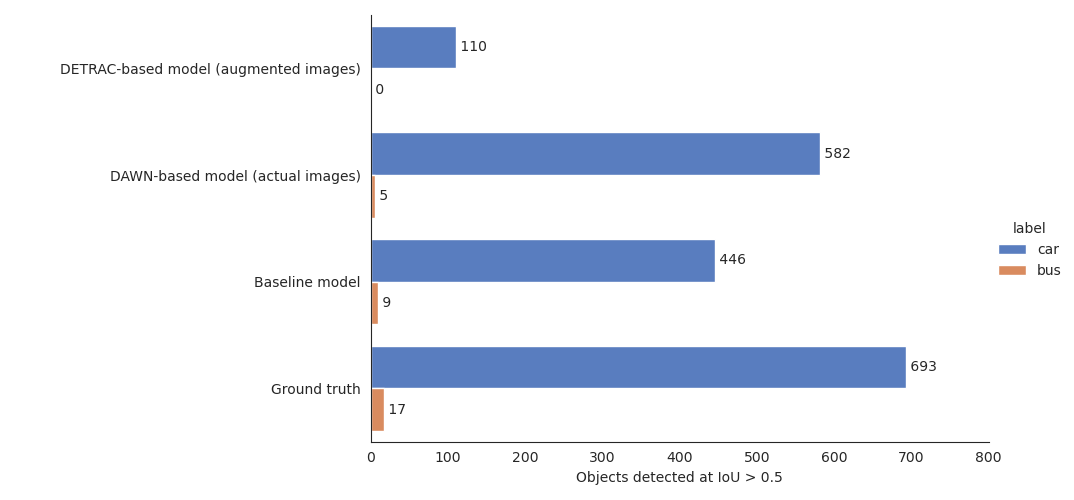
\includegraphics[width=120mm]{object_prediction_iou_0.5.png} \\ 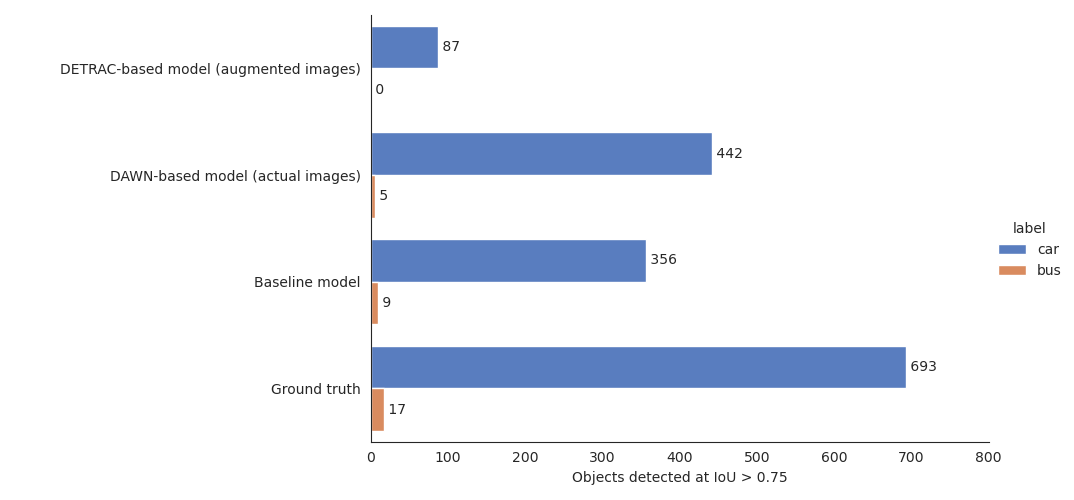
\includegraphics[width=120mm]{object_prediction_iou_0.75.png} \\ 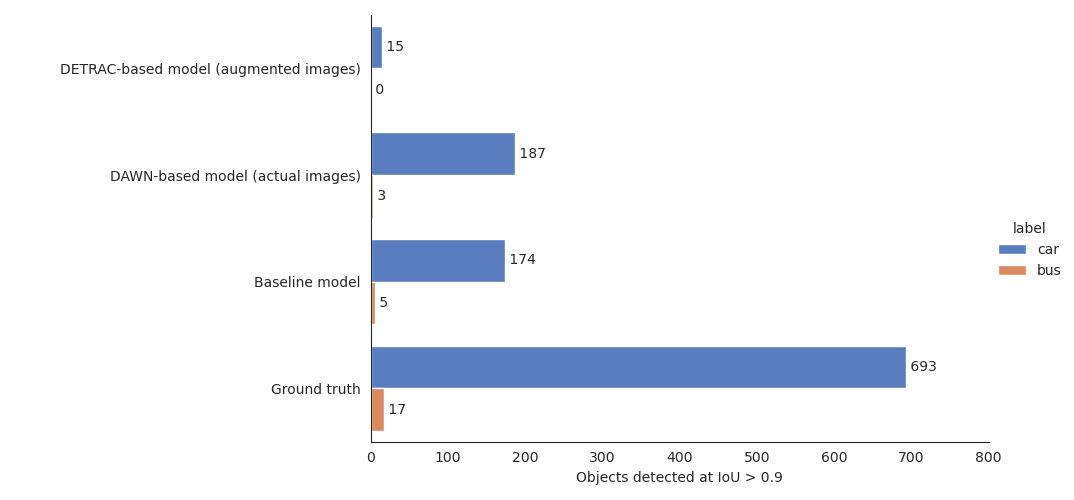
\includegraphics[width=120mm]{object_prediction_iou_0.9.png}
	\end{tabular}
	\caption{Object detection for IoU $ > 0.5$, IoU $ > 0.75$ and IoU $ > 0.9$ respectively.}
	\label{fig:iou-thresholds}
	\end{figure}

\section{Conclusion}

We have found that the DAWN-based model consistently outperforms the baseline model for the detection of cars in traffic images of adverse weather conditions. For the detection of buses, we observed some training effects in both the DAWN and DETRAC models. Yet, with a mere 17 ground truth buses in 98 images these observations provide too little conclusive evidence. From our experiments, we cannot confirm the first research question (RQ\ref{rq1}). However, we did find some confirming evidence for the second of our research questions (RQ\ref{rq2}). This means that training a standard YOLO\small{v8} model with actual images of traffic in adverse weather conditions is likely to provide models with better prediction accuracy. Finally, we did not find conclusive evidence for the third research question (RQ\ref{rq3}). Our experiments could not establish an approximate equivalence in terms of prediction accuracy between the DAWN-based model and the DETRAC-based model. In short, our study does not support the assertion that training with augmented images is a viable substitute for training with actual images. 

\begin{appendices}
	\section{Research method}
	
	The selection and partitioning of image sets is schematically depicted in Figure \ref{fig:schema}.
	
	\begin{figure}[H]
		\centering
		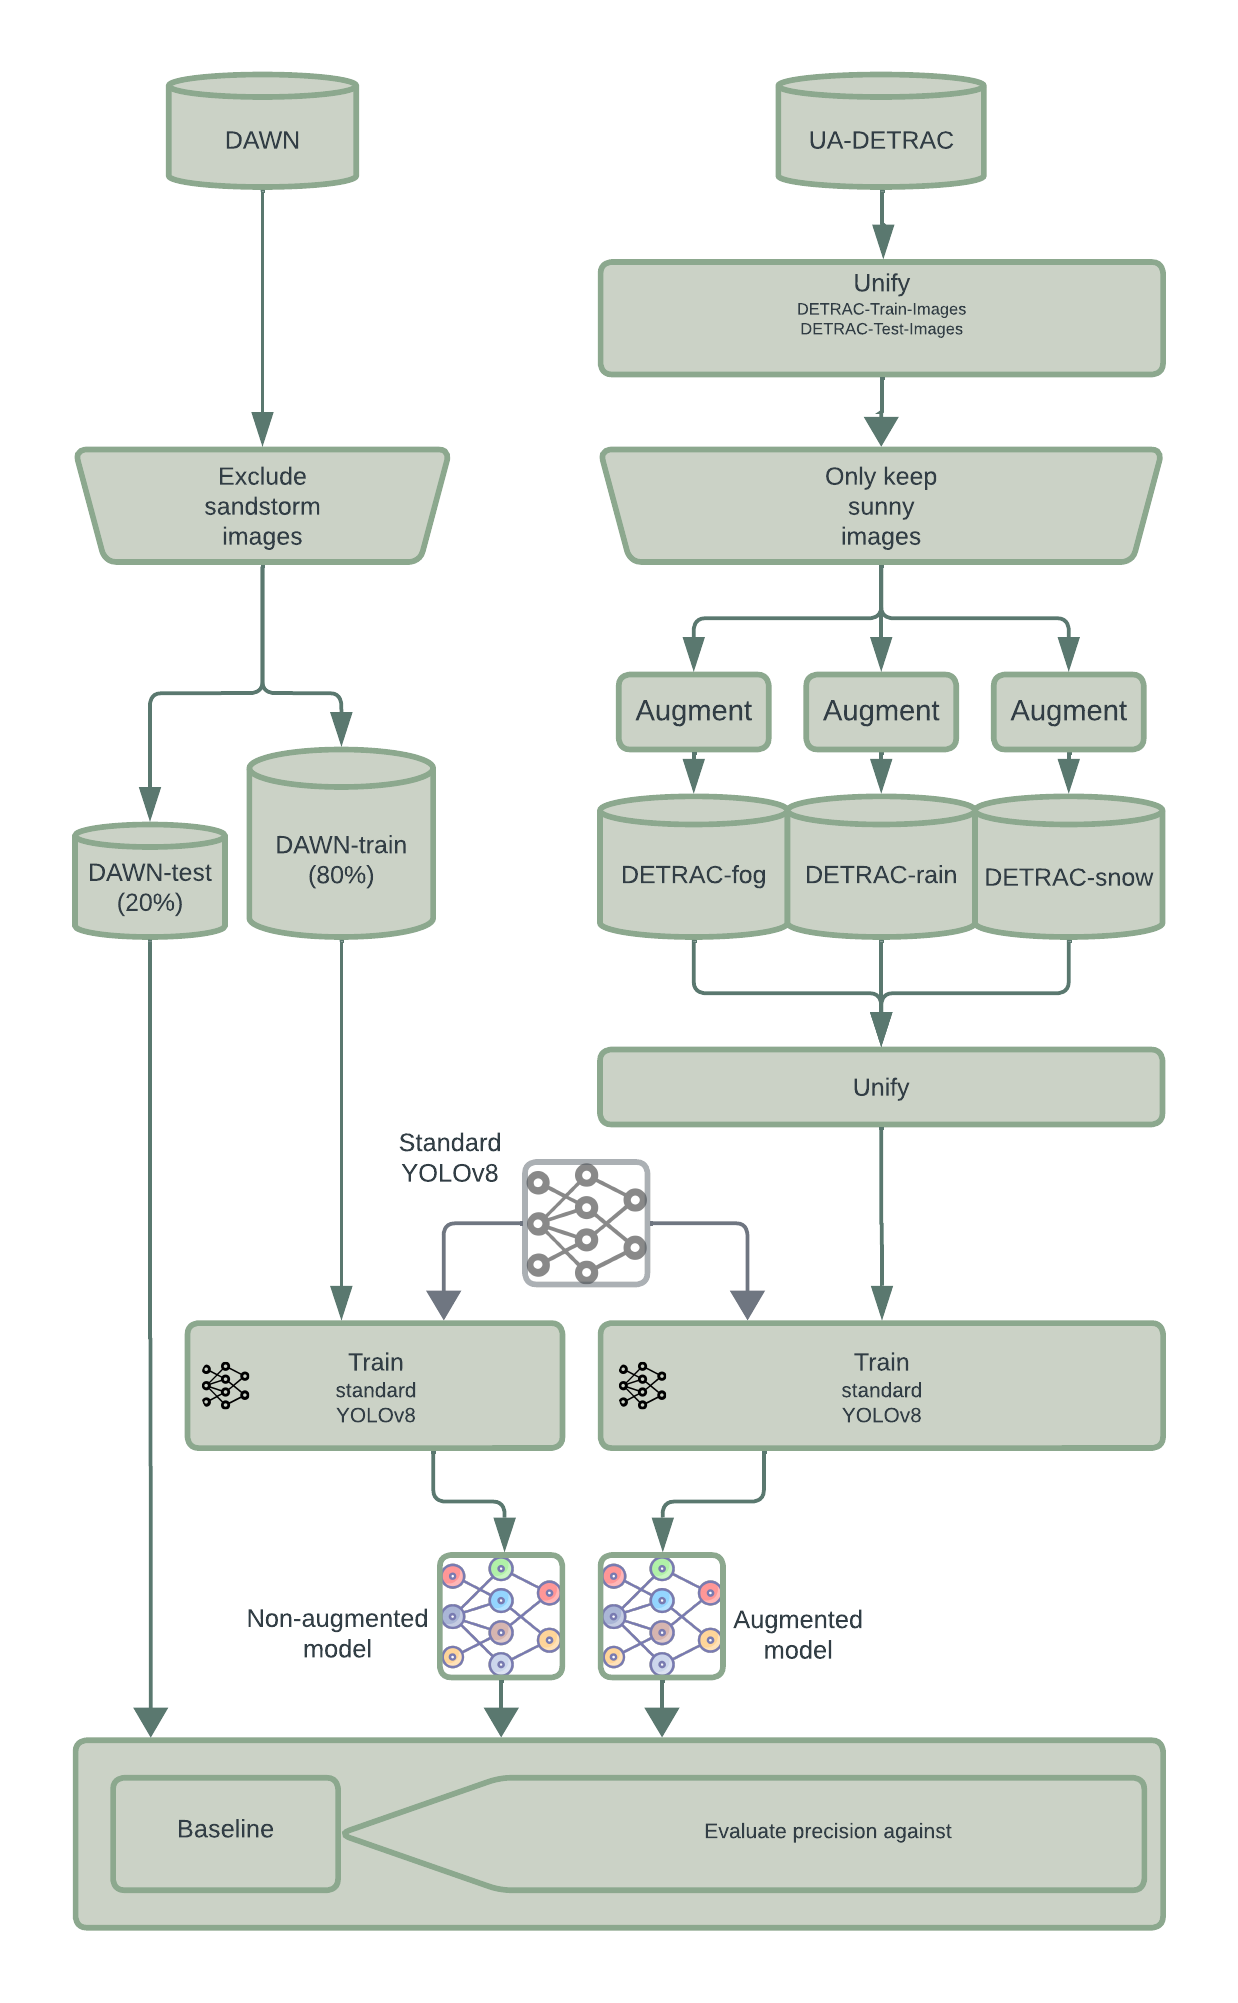
\includegraphics[width=100mm]{Proposal_diagram.png}
		\caption{Schematic representation of the research method.}
		\label{fig:schema}
	\end{figure}
	
\end{appendices}


\printbibliography

\end{document}
